\documentclass[11pt]{article}

% \usepackage[sort]{natbib}
\usepackage[style=verbose]{biblatex}
\usepackage{fancyhdr}
\usepackage{graphicx,caption,subcaption,color,float} %Graphics stuff
\usepackage{hyperref,amssymb,amsmath, amsfonts, amsthm, enumerate, bm}
\usepackage{placeins, cancel, wrapfig, xcolor, array, multirow, booktabs, algorithm, algpseudocode} 
\usepackage[margin=0.9in]{geometry}
\usepackage{ulem}
\graphicspath{ {figs/} }
\bibliography{references}

% you may include other packages here (next line)
\usepackage{enumitem}
\usepackage{dirtytalk}
\usepackage{pythonhighlight}


%----- you must not change this -----------------
\topmargin -1.0cm
\textheight 23.0cm
\parindent=0pt
\parskip 1ex
\renewcommand{\baselinestretch}{1.1}
\pagestyle{fancy}
\renewcommand{\theenumi}{\Alph{enumi}}
\makeatletter
\newcommand{\distas}[1]{\mathbin{\overset{#1}{\kern\z@\sim}}}%
\newsavebox{\mybox}\newsavebox{\mysim}
\newcommand{\distras}[1]{%
  \savebox{\mybox}{\hbox{\kern3pt$\scriptstyle#1$\kern3pt}}%
  \savebox{\mysim}{\hbox{$\sim$}}%
  \mathbin{\overset{#1}{\kern\z@\resizebox{\wd\mybox}{\ht\mysim}{$\sim$}}}%
}
\makeatother
%----------------------------------------------------

% enter your details here----------------------------------
\lhead{}
\chead{}
\rhead{}
\lfoot{}
\cfoot{}
\rfoot{}
\setlength{\fboxrule}{4pt}\setlength{\fboxsep}{2ex}
\renewcommand{\headrulewidth}{0.4pt}
\renewcommand{\footrulewidth}{0.4pt}


\title{Homework 1}
\author{Pan Du}

\begin{document}

\maketitle

\textbf{Problem 1:}
In order to let Katz centrality converge, the term $(\mathbf{I}-\alpha\mathbf{A})^{-1}$ must have value, which means $\mathbf{I}-\alpha\mathbf{A}$ is invertible. So we need $det(\mathbf{I}-\alpha\mathbf{A}) \neq 0$. Note that if $\mathbf{A}$ is a singular matrix, we have $$
det(\mathbf{I}-\alpha\mathbf{A}) = 0 \Rightarrow det(\mathbf{A}-\frac{1}{\alpha}\mathbf{I}) = 0 \Rightarrow \alpha = \frac{1}{\lambda}
$$
where $\lambda$ is the eigen value of matrix A. $\alpha$ takes the minimum value when $\lambda$ is the largest eigen value. So to ensure $\mathbf{A}$ is not sigular, we should let $\alpha$ smaller than this minimum value, in other words:
$$
\alpha < \frac{1}{\lambda_1}
$$
Where $\lambda_1$ is the leading eigen value of matrix A. 


    

\clearpage


\textbf{Problem 2:}
Using the "walk" concept, you will start from node $v_i$ and go two hops, then count the distinct paths that end in node $v_j$, which should be equal to the number of common neighbours. Mathematically:
We have adjacency matrix $\mathbf{A}$, we want to check the common neighbourhood of node $v_i$ and $v_j$. The number of common neighbour equalls to the element $\mathbf{A}^2_{ij}$ which can be calculated as:
$$
    |N(v_i)\cap N(v_j)| = [\mathbf{A}^2]_{ij} = \sum_{k}{\mathbf{A}_{ik}\mathbf{A}_{kj}}
$$


\clearpage

\textbf{Problem 3:}\\
A. Code written in python and pushed to github\\
First, we calculate the Jaccard similarity of each pair of nodes. 
\begin{python}
# calculate the Jaccard similarity between every pair of nodes 
S = np.zeros((len(nodes),len(nodes)))
for i in range(len(nodes)):
    for j in range(len(nodes)):
        NinNj = np.array(A.todense()[:,i])*np.array(A.todense()[:,j]) # calculate the intersection of N(vi) and N(vj)
        NiuNj = np.array(A.todense()[:,i])+np.array(A.todense()[:,j]) # calculate the union of N(vi) and N(vj)
        S[i,j] = len(np.nonzero(NinNj)[0])/len(np.nonzero(NiuNj)[0]) # put into S matrix
\end{python}


Then we create another graph where the edges will be node "Ginori" connecting to all the nodes in the graph. The value on the edges will be the corresponding similarity. 

\begin{python}
# creating a copy of original graph 
G2 = nx.create_empty_copy(G, with_data=True)
old_edges = copy.deepcopy(G.edges())
new_edges, metric = [], []

# set new edges according to Similarity to node "Ginori"
for i in range(len(G2.nodes)):
    G2.add_edge('Ginori', list(nodes)[i])
    # print(f"({u}, {v}) -> {p:.8f}")
    new_edges.append(('Ginori', list(nodes)[i]))
    metric.append(S_dict[list(nodes)[i]])
\end{python}


B. This is the plot:

\begin{figure}[h]
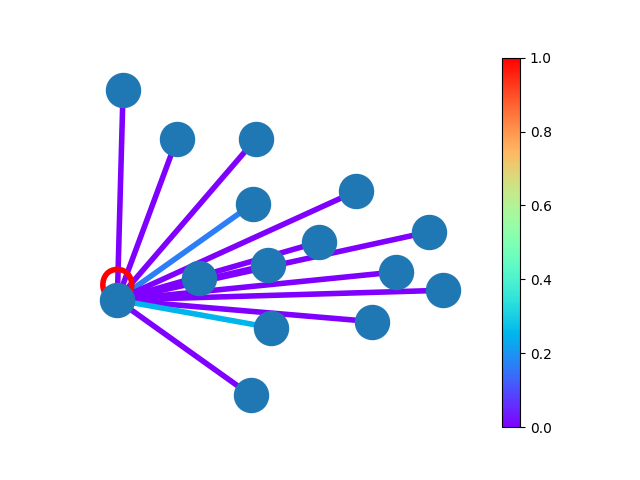
\includegraphics[width=8cm]{Jaccard.png}
\end{figure}
\clearpage



\end{document}